\documentclass[a4wide,12pt]{report}
\usepackage[utf8]{inputenc}
\usepackage[IL2]{fontenc}
\usepackage{listings}
\usepackage{amssymb}
\usepackage{amsmath}
\usepackage{url}
\usepackage{graphicx}
\usepackage[czech]{babel}
%\usepackage{fullpage}
\usepackage[top=22mm, bottom=30mm, left=35mm, right=25mm]{geometry}
\usepackage{tikz}
\usepackage{subfig}
\usepackage{float}
\hyphenation{NetLogo}
\title{sds}
\author{Marek Bryša}
\date{Brno 2011}
\begin{document}
\tableofcontents

\chapter*{Úvod}
\addcontentsline{toc}{chapter}{Úvod}
co,jak,proc\\
zduvodneni "pro vyuku mikroekonomie"\\
o sitovem marketingu obecne\\
$\pm$1s
\chapter{Prodejní síť Oriflame}
\section{Historie firmy Oriflame}
Firma Oriflame byla založena v roce 1967 ve Švédsku bratry Jonasem a Robertem Jochnick. Cílem bylo nabídnout lidem přirozenou a přírodní péči o svou pleť. Místo aby nákladně budovali kamenné obchody, rozhodli se dostat prodej přímo do domovů a využít tak vrozenou podnikavost lidí. Tento základní koncept zůstáva po více než 40 let nezměněn. V roce 1990, po po pádu železné opony, firma expanduje po střední a východní Evropě a zakládá pobočku i v České republice. V roce 2001 dosahuje počet kosmetických poradců jednoho miliónu a obrat téměř 450 miliónů EUR.

Sortiment je opravdu široký, katalog obsahuje přes 1500 výrobků v cenách přibližně od 50 do 1000 Kč. Většina typů produktů obsahuje několik cenou a kvalitou odlišených řad. Celkově lze říci, že zákazník má možnost nákupu komplexní péče s téměř libovolným rozpočtovým omezením.
\section{Podmínky síťového prodeje}
V této části popíšeme fungování sítě Oriflame na českém trhu. V jiných zemích se mohou zejména parametry mírně lišit. Prodejcem (v terminologii Oriflame \emph{poradcem}) se zájemce stane vyplněním jednoduchého formuláře a zaplacením poplatku 99 Kč. Tím získá možnost výdělku následujícími způsoby:
\begin{enumerate}
\item Nákupem kosmetických výrobků v centrech Oriflame nebo na objednávkou přes internet za tzv. nákupní ceny, které jsou o 30\% nižší než prodejní (katalogové) ceny. Prodejce tak realizuje 30\% marži z prodeje sobě a svým zákazníkům (typicky rodině a známým).
\item Plnou hodnotu tzv. \emph{slevy z obratu} svého vlastního prodeje.
\item Budováním skupiny poradců, které k Oriflame přivedl, tzv. \emph{sponzoroval}. Pak mu náleží rozdíl mezi svou slevou z obratu a slevou z obratu lidí, které k Oriflame přivedl a jejich skupin.
\end{enumerate}
Tento systém slouží jako motivace lidí pro rozšíření prodejní sítě. Je založen na očekávaní vysokého výdělku v budoucnosti. Firma ve svých materiálech jako příklad uvádí lineární růst výdělku pro poradce z prodeje a exponenciální ze sponzorování.

Rok je rovnoměrně rozdělen na 17 období, které odpovídají vydáním katalogů výrobků. Poradce, který podal v předchozích třech obdobích alespoň jednu objednávku, obdrží sadu tiskovin zdarma, jinak je pro něj téměř nutnost si tištěný katalog zakoupit za TODO:cena katalogu.

Firma dále nabízí pro začínající poradce ve čtyřech krocích motivaci ve formě věcných darů za splnění určitých objemů obratu, např. v prvním kroku za obrat 1250 Kč tašku, průvodce péčí o pleť a krém v celkové hodnotě 510 Kč.

Také jsou k dispozici úvěry do výše 7000 Kč na zaplacení za zobží, které hodlá poradce dodat zákazníkum a nemusí tak od nich vybírat peníze předem.

Oriflame poskytuje garanci vrácení peněz do 30 dnů od nákupu výrobku bez udání důvodu a to i v případě, že výrobek obsahuje minimálně 80\% původního objemu.
\subsection{Skupiny a slevy z obratu}
Každému výrobku jsou v ceníku přiděleny čtyři hodnoty:
\begin{description}
\item[PC] Doporučená prodejní cena spotřebitelům.
\item[NC] Nákupní cena včetně DPH. Za tu poradci mohou zobží zakoupit v centrech Oriflame.
\item[OO] Obchodní obrat. Typicky je roven nákupní ceně bez DPH. V případě nespotřebních produktů (např. kartáč na vlasy, houba na mytí) je ještě přibližně poloviční.
\item[BO] Bodové ohodnocení. Na inflaci nezávislý počet bodů, které poradce nákupem zboží získá. V současnoti odpovídá přibližně 13,80 Kč obchodního obratu.
\end{description}
Výjimku tvoří např. tiskoviny, vzorky a oblečení s logem Oriflame, které mají pouze nákupní cenu,  nejsou určeny k dalšímu prodeji a slouží jen jako pomůcka pro poradce.

Poradce dále získá body všech lidí které přivedl a těch pod nimi. Na konci každého katalogového období dochází k vyhodnocení. Sečtou se všechny body a podle tabulky \ref{tab:perc_level} se určí procentní úroveň.
\begin{table}[h]
\begin{center}
\begin{tabular}{|l|c|c|c|c|c|c|c|}
\hline
body & $\geq$200 & $\geq$600 & $\geq$1200 & $\geq$2400 & $\geq$4000 & $\geq$6600& $\geq$10000\\\hline
úroveň & 3\% & 6\% & 9\% & 12\% & 15\% & 18\% & 21\%\\\hline
\end{tabular}
\end{center}
\caption{Určení procentní úrovně}
\label{tab:perc_level}
\end{table}
Toto se provede i pro všechny podskupiny. Poradce pak získá za každou podskupinu: obchodní obrat skupiny $\cdot$ (procentní úroveň poradce $-$ procentní úroveň skupiny). Tím je zajištěno, že člověk, který se stal poradcem Oriflame později, ale je schopnější, může dosáhnout vyššího výdělku než ten, kdo jej přivedl. Poradce také obdrží přímo podle své procetní úrovně slevu ze svého vlastního prodeje.

Všechny tyto peníze poradce dostane na účet. Podmínkou je, že jeho vlastní prodej musí dosáhnout 100 bodů. To firma zdůvodňuje tím, že poradce musí být sám schopným prodejcem, aby mohl učit ostatní.

Při dosažení 12\% úrovně se poradce stává tzv. manažerem, při 21\% direktorem. Za to má možnost získat věcné i finanční prémie, účast na školeních aj. V případě, že osoba na 21\% úrovní sponzoruje někoho, kdo jí dosáhl také, stanovuje se procetní rozdíl úrovní na 3\%.
\\TODO: priklad grafu skupiny?
\\\tikz
\node {Computational Complexity\\dsa} % root
child { node {Computational Problems}
child { node {Problem Measures} }
child { node {Problem Aspects} }
child { node {Problem Domains} }
child { node {Key Problems} }
}
child { node {Computational Models}
child { node {Turing Machines} }
child { node {Random-Access Machines} }
child { node {Circuits} }
child { node {Binary Decision Diagrams} }
child { node {Oracle Machines} }
child { node {Programming in Logic} }
}
child { node {Measuring Complexity}
child { node {Complexity Measures} }
child { node {Classifying Complexity} }
child { node {Comparing Complexity} }
child { node {Describing Complexity} }
}
child { node {Solving Problems}
child { node {Exact Algorithms} }
child { node {Randomization} }
child { node {Fixed-Parameter Algorithms} }
child { node {Parallel Computation} }
child { node {Partial Solutions} }
child { node {Approximation} }
};

\chapter{Popis modelu}
V této kapitole se budeme věnovat popisu modelu sítě Oriflame z technického a ekonomického pohledu. Dojde i k částečnému prolnutí se implementací modelu na počítači, což je nutné, aby si jej čtenář mohl v případě potřeby snáze upravit.
\section{Technický popis}
Pro vytvoření experimentálního modelu bylo zvoleno prostředí NetLogo\footnote{NetLogo, \url{http://ccl.northwestern.edu/netlogo/}} ve verzi 4.1.3. Je to oteřený a volně šiřitelný software umožňující snadnou tvorbu agentových a systémově-dynamických modelů. Běh modelu zahrnuje zpravidla dvě části:
\begin{enumerate}
\item Inicializace (setup). Zde se nastaví všechny proměnné na výchozí hodnoty, většinou také dojde k vygenerování náhodných parametrů a vztahů pro jednotlivé agenty.
\item Vlastní běh. Ten probíhá v opakovaných oddělených krocích. V každém z nich dojde k projevu chování agentů a tím změně promenných, vztahů mezi agenty atd.
\end{enumerate}
V tomto modelu se pracuje zejména s agenty \texttt{person}, obousměrným vztahem \texttt{friend} a jednosměrným \texttt{sponsor}.
\section{Ekonomický popis}
\subsection{Generování sociálních vazeb}
Je nutné, aby model věrně zachytil sociální vztahy ve společnosti. Každý agent ma jistý okruh přátel, kterým může prodávat kosmetické výrobky a nabídnout jim členství v prodejní síti. Model obsahuje konstanty \texttt{number-of-persons} a \texttt{number-of-friendships}. První značí počet vygenerovaných osob, druhá počet náhodných přátelství mezi nimi. Je nutné aby graf tovřil jednu komponentu, protože na světě prakticky neexistují uzavřené a s nikým nekomunikující skupiny lidí. To je zajištěno tak, že ihned po vygenerování všech lidí každý postupně vytvoří přátelství s někým, kdo už nějaké má. Tím vzniká mírné vychýlení oproti jinak normálnímu rozdělení počtu přátelství na osobu, které je ale vzhledem k počtu dále přidaných přátelství zanedbatelné. Na obrázku \ref{fig:hist_fr} jsou histogramy jednoho běhu generování přátelství pro $\texttt{number-of-persons}=\texttt{number-of-friendships}=300$ před a po přidání náhodných přátelství.\\
\begin{figure}[h]
  \centering
  \subfloat[Před přidáním náhodných]{\label{fig:hist_fr_v1}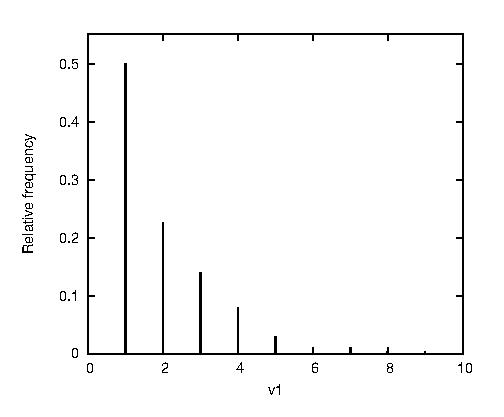
\includegraphics[width=0.5\textwidth]{hist_fr_v1.eps}}                
  \subfloat[Po přidání náhodných]{\label{fig:hist_fr_v2}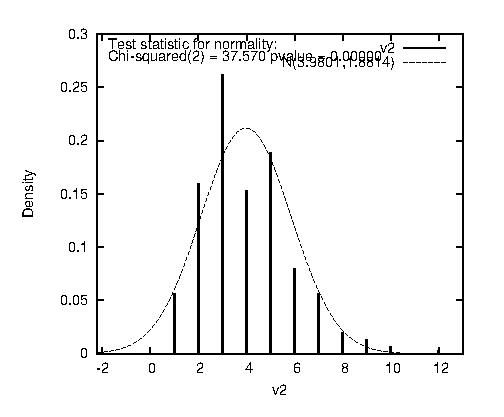
\includegraphics[width=0.5\textwidth]{hist_fr_v2.eps}}
  \caption{Histogram počtu přátelství}
  \label{fig:hist_fr}
\end{figure}
%\begin{center}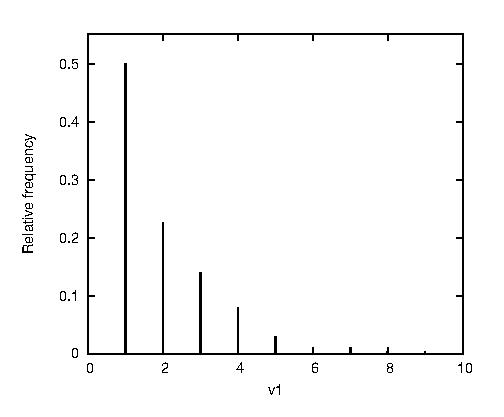
\includegraphics{hist_fr_v1.eps}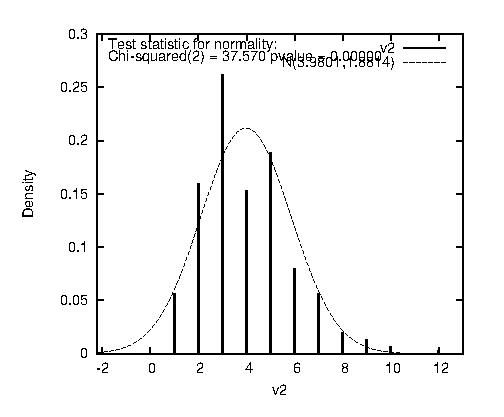
\includegraphics{hist_fr_v2.eps}\end{center}
\subsection{Prostředí}
Agenti jsou generování v izolovaném prostředí. Na začátku je jeden z nich určen jako zdrojový a od něj se pak síť může postupně po jednotlivých kolech šířit. Je možne také zapnout volbu \texttt{random-join?}, která znamená, že v každém kole je nabídnuto členství jednomu náhodnému agentovi --- nečlenovi. To modeluje případ, kdy se poradci snaží o nábor lidí např. u stánků.

Dále jsou přítomny tyto za běhu měnitelné konstanty:
\begin{description}
\item[\texttt{margin}] Marže pro prodejce.
\item[\texttt{monthly-fee}] Poplatek za členství placený v každém kole. Firma Oriflame jej nevybírá, je tedy určen spíše pro experimenty.
\end{description}
\subsection{Vlastnosti agenta \texttt{person}}
\label{sec:vl_agenta}
Agent \texttt{person} představuje v modelu jednoho člověka. Má tyto důležité vlastnosti:
\begin{description}
\item[\texttt{consupmtion}] Množství peněz, které daná osoba během jednom období může utratit za kosmetické výrobky, které je možno koupit v síti Oriflame. Je to ekvivalent rozpočtového omezení a považuje se za konstantní. Ve výchozím nastavení je generováno jako:
$$\max\{100,\texttt{random-normal(1000,500)}\}$$
Tj. náhodná hodnota z normálního rozdělení se střední hodnotou 1000, rozptylem 500, zdola omezená 100 (spořeba nižší než 100 by byla nevýznamná).
\item[\texttt{netmember?}] Značí, zda je agent členem sítě --- poradcem.
\item[\texttt{be-point}] Bod ukončení činnosti. Členstvím v síti vznikají každému náklady. Tvoří je explicitní např. výdaje za cestu k zakazníkům a implicitní za čas obětovaný této práci. Obecně lze říci, že implicitní složka bude tím vyšší, čím lépe na daný člověk placené hlavní zaměstnání. A tím se také zvyšuje jeho rozpočtové omezení. Proto existuje závislost mezi consumption a be-point vyjádřená:
$$\max\{\texttt{consumption}\cdot 0.5,\texttt{consumption}\cdot\texttt{random-normal(1,0.5)}\}$$
\end{description}
\subsection{Chování agenta \texttt{person}}
Chování vychází z jednoduché racionálni úvahy --- vyplatí se do sítě vstoupit a zůstat v ní? Lze jej tedy rozdělit na dvě části: podmínku vstupní a podmínku setrvání.
\subsubsection{Vstupní podmínka}
Pokud je agentovi nabídnuto členství, přijme ho jestliže
\[(\texttt{myrev} + \texttt{avg-exp-rev}) \cdot (1+\texttt{d-margin}) \geq \texttt{be-point} + \texttt{monthly-fee}.\]
\begin{description}
\item[\texttt{myrev}] je očekávaný příjem z přímeho prodeje přátelům agenta. Vypočítá se jako \[\sum_{p\in F}(\texttt{consumption}_p\cdot\texttt{margin}),\]
kde $F$ je množina přátel. Pokud některému z nich může zboží dodávat více poradců, je spotřeba rozdělena rovnoměrně mezi ně.
\item[\texttt{avg-exp-rev}] je očekávaný příjem ze sponzoringu a skupin. Protože v rozhodování člověka je jistá setrvačnost, je dán jako průměr posledních deseti skutečných příjmů z této činnosti. Při inicializaci je naplněn hodnotami
\[ 0.09\cdot (\sum_{p\in F}\texttt{consumption}_p)\cdot |F|^{1.3}.\]
To odpovídá odhadu uváděnému při nabídce členství v síti.
\item[\texttt{d-margin}] je rozdíl mezi současnou \texttt{margin} a tou při posledním odchodu agenta ze sítě, nejméně 0. To proto, že pokud se marže od posledního pokusu o nábor člena zvýšila, bude to použito jako argument, v opačném případě spíše zamlčeno.
\end{description}
\subsubsection{Podmínka setrvání}
Ta je dána velmi podobně:
\[ \texttt{avg-exp-rev} + \texttt{my-rev} \geq \texttt{be-point} + \texttt{monthly-fee} \]
\texttt{my-rev} v tomto případě již není odhad, ale skutečná hodnota.
%
%
%
\chapter{Analýza a experimenty}
V této kapitole budeme provádět experimenty na modelu prodejní sítě Oriflame a analyzovat jejich výsledky. Pokud nebude uvedeno jinak pracujeme s výchozím modelem a základními parametry:\\
$\texttt{number-of-persons}=\texttt{number-of-friendships}=300$, \\
$\texttt{margin}=0.3,\\\texttt{monthly-fee}=100$ a\\
vlastnosti agenta \texttt{person} uvedené v sekci \ref{sec:vl_agenta}.

Data budou získána pomocí nástroje BehaviorSpace obsaženého v programu NetLogo. Ten umožňuje opakovaný běh modelu se stejnými náhodnými složkami, ale při různých parametrech, čímž lze získat velké a robustní datové soubory.

K měření budou sloužit mimo jiné tyto veličiny:
\begin{description}
\item[\texttt{network-fee-revenue}] Příjem firmy z poplatků.
\item[\texttt{network-sale-revenue}] Příjem firmy z prodeje výrobků (za nákupní ceny).
\item[\texttt{revenue}] Součet předchozích dvou.
\item[\texttt{scost}] Náklady na výplatu sponzoringu a skupin.
\end{description}
Ke statistické analýze bude využit ekonometrický software GRETL\footnote{Gnu Regression, Econometrics and Time-series Library, \url{http://gretl.sourceforge.net/}} verze 1.9.1 a tabulkový procesor Gnumeric\footnote{Gnumeric --- The Gnome Office Spreadsheet, \url{http://projects.gnome.org/gnumeric/}} 1.10.14.
\section{Šíření sítě}
Zde se budeme zkoumat šíření sítě a její výsledné vlastnosti. 
\subsection{Průběh šíření}
Bylo provedeno 100 nezavislých náhodných běhů. Podmínkou ukončení je stabilizace sítě, tj. rovnost dvou po sobě následujících \texttt{revenue}. Získaná data jsou v přiloženém souboru \texttt{spread1.csv}. Z nich odvozené popisné statistiky jsou v tabulce \ref{tab:spread1_desc}.
\begin{table}[h]
  \begin{center}
  \begin{tabular}{|r|r|r|r|}
  \hline
  Statistika&Počet členů na konci	&Maximum členů	&Počet kol do stabilizace\\\hline
  Průměr	&81.47	&217.2	&24.17\\
  Medián	&82	&218	&24\\
  Std. odchylka	&3.83	&6.67	&2.09\\
  Minimum	&72	&202	&20\\
  Maximum	&92	&234	&29\\\hline
  \end{tabular}
  \end{center}
  \caption{Popisné statistiky pro \texttt{spread1}}
  \label{tab:spread1_desc}
\end{table}
Vidíme, že průměrný běh trval 24 kol. Členy sítě se maximálně stalo 217 osob z 300 a nakonec zůstalo 81, tedy přibližne čtvrtina. Časová řada počtu členů jednoho vybraného běhu je vidět na grafu \ref{fig:spread1_run}.
\begin{figure}[h]
  \centering
  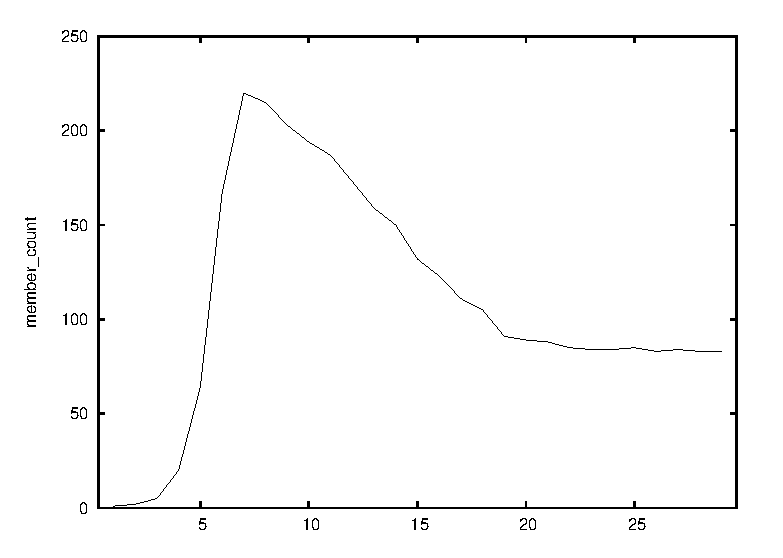
\includegraphics{member_count.eps}
  \caption{Vybraný běh experimentu \texttt{spread1}}
  \label{fig:spread1_run}
\end{figure}
%\begin{center}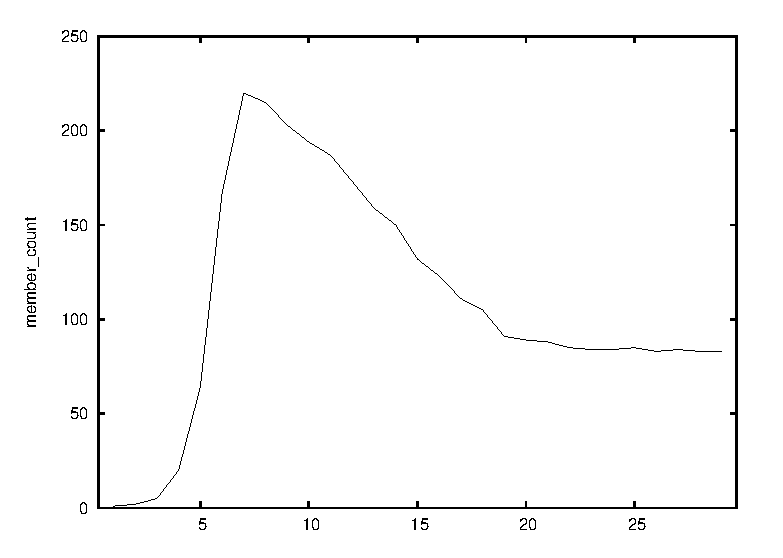
\includegraphics{member_count.eps}\end{center}
Je patrné, že síť se z počátku rychle rozrůstá díky velkým očekáváním. Ta ale nejsou většinou naplňena a dochází k postupnému úbytku.
\subsection{Vlastnosti agentů}
Nabízí se otázka, jakou vlastnost mají agenti, kteří v síti zůstali. Jedním důvodem může být nadprůměrný počet přátel. Za stejných podmínek jako v předchozím případě sestavíme experiment. Výsledkem běhu je průměrný počet přátel pro člena sítě a pro všechny osoby. Data jsou k dispozici v souboru \texttt{spread2.csv}. Popisné statistiky jsou v tabulce \ref{tab:spread2_desc}.
\begin{table}[H]
  \begin{center}
  \begin{tabular}{|r|r|r|r|}
  \hline
  Statistika&Průměrný počet přátel pro člena	&Průměrný počet přátel pro všechny\\\hline
  Průměr	&5.44	&3.98\\

  Variance	&0.03	&0.00\\\hline
  \end{tabular}
  \end{center}
  \caption{Popisné statistiky \texttt{spread2}}
  \label{tab:spread2_desc}
\end{table}
Hypotéza: $M_1=M_2 ~ \bot ~ M_1>M_2$\\
P-hodnota testové statistiky $T = 9.51\cdot 10^{-97}$\\
Jednoznačně tedy zamítáme nulovou hypotézu a je zřejmé, že stálí členové sítě mají nadprůměrný počet přátel.

Druhým důvodem může být malý \texttt{be-point}, což způsobí výhodnost členství. Experiment provedeme stejným způsobem jako u počtu přátel. Statistiky vidíme v tabulce \ref{tab:spread3_desc}. Výsledky lze nalézt v souboru \texttt{spread3.csv}.
\begin{table}[H]
  \begin{center}
  \begin{tabular}{|r|r|r|r|}
  \hline
  Statistika&Průměrný \texttt{be-point} pro člena	&Průměrný \texttt{be-point} pro všechny\\\hline
  Průměr	&533.45	&1051.82\\

  Variance	&1279.18	&1896.18\\\hline
  \end{tabular}
  \end{center}
  \caption{Popisné statistiky \texttt{spread3}}
  \label{tab:spread3_desc}
\end{table}
Hypotéza: $M_1=M_2 ~ \bot ~ M_1>M_2$\\
P-hodnota testové statistiky $T = 3.06\cdot 10^{-109}$\\
Nade vší pochybnost opět zamítáme možnost rovnosti průměrů. Členové tedy maji obecně podprůměrný \texttt{be-point}.

Z těchto dvou experimentů je patrné, že poradci se rekrutují z řad lidí s nižším příjmem a velkým počtem přátel. Model z tohoto pohledu věrně vystihuje realitu, neboť ve společnosti tuto skupinu tvoří převážně studenti a např. rodiče na mateřské dovolené --- největší část poradců Oriflame.
\section{Vliv náborových akcí}
Jak již bylo uvedeno, někteří poradci z vlastní iniciativy pořádají náborové akce, kde se snaží přivést k Oriflame i lidi mimo své přátele. Model to simuluje tak, že se v každém kole nabídne členství jednomu náhodnému nečlenovi. Budeme zjišťovat, zda-li to má význam pro počet členů po stabilizaci. Provedeme dva experimenty, první s \texttt{random-join?} vypnutým a druhý se zapnutým. V obou bude celkem 226 běhů modelu s \texttt{number-of-friendships} zvyšujícím se od 50 do 500 po krocích velikosti 2. Data jsou uložena v souborech \texttt{random-join1.csv} a \texttt{random-join2.csv}. Výsledné bodové grafy jsou na obrázku \ref{fig:random-join}. Metodou nejmenších čtverců byly nalezeny tyto regresní přímky:
\begin{figure}[h]
  \centering
  \subfloat[\texttt{random-join?} vypnuto]{\label{fig:random_join1}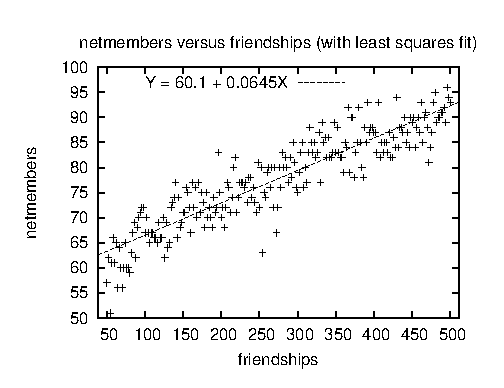
\includegraphics[width=0.5\textwidth]{random-join1-1.eps}}                
  \subfloat[\texttt{random-join?} zapnuto]{\label{fig:random_join2}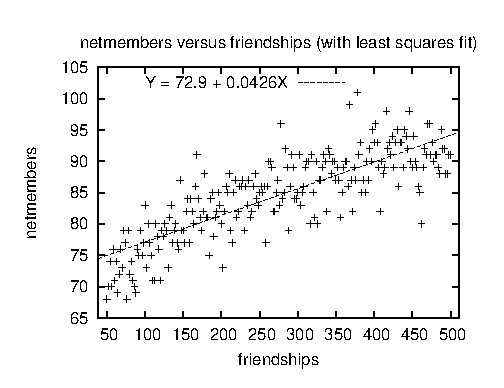
\includegraphics[width=0.5\textwidth]{random-join2-1.eps}}
  \caption{Bodový graf experimentů \texttt{random-join} s OLS přímkou}
  \label{fig:random-join}
\end{figure}
\begin{itemize}
\item \texttt{random-join?} vypnuto\\
\begin{gather}
\widehat{\rm netmembers} = 
\underset{(0.61341)}{60.0865}
+\underset{(0.0020152)}{0.0644801}\,\mbox{friendships}
 \notag \\
T = 226 \quad \bar{R}^2 = 0.8197 \quad F(1,224) = 1023.8 \quad \hat{\sigma} = 3.9530 \notag
\end{gather}

\item \texttt{random-join?} zapnuto\\
\begin{gather}
\widehat{\rm netmembers} = 
\underset{(0.62107)}{72.8508}
+\underset{(0.0020404)}{0.0426021}\,\mbox{friendships}
 \notag \\
T = 226 \quad \bar{R}^2 = 0.6591 \quad F(1,224) = 435.94 \quad \hat{\sigma} = 4.0024 \notag
\end{gather}
\end{itemize}
Z rovnic vidíme, že náborové akce jsou zvlášť výhodné pro skupiny lidí s nižšími počty přátel. Existuje tam možnost vzniku slabých článků, které zabrání dalšímu šíření sítě. Bez zajímavostí není, že dojde k průniku přímek při $\texttt{number-of-friendships}=584$, což přibližne odpovídá průměrnému počtu přátel $5,84$. Pro poradce z toho plyne doporučení, že pokud je počet přátelství v jejich okolí (za předpokladu jisté homogenity) vyšší než tato hodnota, není pro ně výhodné pořádat nábory, protože síť si ke všem najde cestu sama.
\section{Slabé články}
V předchozí části jsme zjistili existenci slabých článků, tj. agetů, přes které síť neprojde a její šíření se zastaví. Zde se je pokusíme identifikovat a objevit jejich společné vlastnosti. Slabý článek (bottleneck) bude určen tímto postupem:
\begin{enumerate}
\item Všem agentům se inicializujeme vlastnost \texttt{invited?} na nepravdu.
\item Necháme síť šířit standardním způsobem bez náhodných náborových akcí do stabilizace, příčemž všem agentům, kterým bylo nabídnuto členství nastavíme \texttt{invited?} na pravdu.
\item Projdeme všechny přátele všech agentů, kterým nebylo nabídnuto členství, a za slabý článek jsou označeni ti, kterým bylo nabídnuto členství.
\end{enumerate}
Zkoumejme nejprve, zda-li existuje závislost mezi \texttt{number-of-friendships} a počtem slabých článků. Sestavíme experiment, který bude \texttt{number-of-friendships} v každém běhu v rozmezí 50 až 500 zvyšovat o 1. Data jsou uložena v souboru \texttt{bottleneck-count.csv}.
\begin{figure}[h]
  \centering
  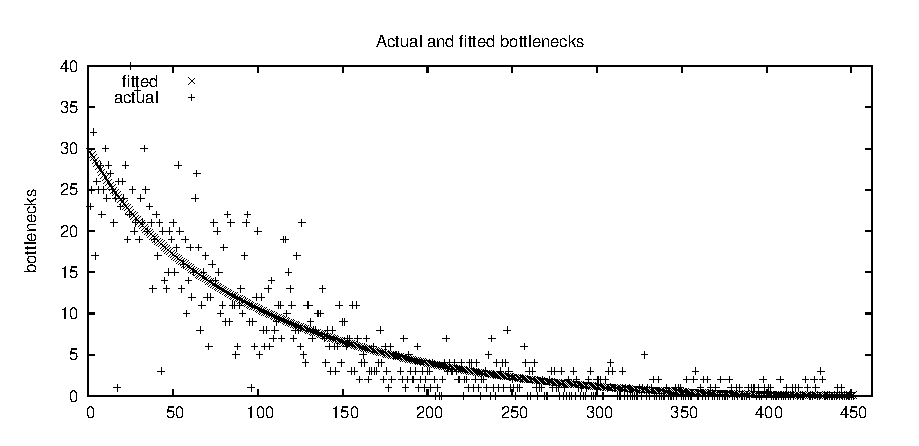
\includegraphics{bottleneck-count.eps}
  \caption{Běh experimentu \texttt{bottleneck-count} s regresní křivkou}
  \label{fig:bottleneck-count}
\end{figure}
\begin{gather}
\widehat{\rm bottlenecks} = 
\underset{(4.2151)}{111.272}
-\underset{(0.98347)}{21.4307}\,\mbox{l\_friendships}
+\underset{(0.0044562)}{0.0440456}\,\mbox{friendships}
 \notag \\
T = 451 \quad \bar{R}^2 = 0.8278 \quad F(2,448) = 1082.9 \quad \hat{\sigma} = 3.3252 \notag
\end{gather}
Vidíme, že s houstnocí sítí vcelku logicky dochází k rychlému poklesu počtu slabých čláků. Ideální hodnotou \texttt{number-of-friendships} pro další zkoumání se jeví 150, kdy již není počet slabých článků tak rozptýlen, ale stále je dost vysoký.

Provedeme experiment se 100 běhy při $\texttt{number-of-friendships}=150$. Zkoumáme průměrný počet přátel a \texttt{be-point} pro všechny a pro slabé články. Výsledné hodnoty jsou v souboru \texttt{bottleneck1.csv}. Popisné statistiky obsahuje tabulka \ref{tab:bottleneck1_desc}. Z ní je patrné, že slabé články mají podprůměrný počet přátel a velmi nadprůměrný \texttt{be-point}. Doporučením pro poradce v případě, že se s nekým takovým setkají, je pokusit se od něj získat alespoň kontakt na jeho známé a tím jej v síti přeskočit.
\begin{table}[h]
  \begin{center}
  \begin{tabular}{|r|r|r|r|r|}
  \hline
   & \multicolumn{2}{|c|}{Prům. počet přátel} & \multicolumn{2}{|c|}{Prům. \texttt{be-point}} \\\hline
	  &všichni	&slabé články	&všichni	&slabé články\\\hline
  Průměr	&3.00	&2.50	&1051.30	&1778.86\\
  Std. odchylka	&0.01	&0.23	&35.17	&260.47\\
  Minimum	&2.98	&2.00	&979.53	&867.00\\
  Maximum	&3.00	&4.00	&1142.78	&2440.33\\\hline
  \end{tabular}
  \end{center}
  \caption{Popisné statistiky \texttt{bottleneck1}}
  \label{tab:bottleneck1_desc}
\end{table}
\section{Reakce na šoky}
\section{Optimální \texttt{margin} a \texttt{monthly-fee}}
\section{Pobídky}
\chapter*{Příručka pro studenty}
\addcontentsline{toc}{chapter}{Příručka pro studenty}
\section{velky model}
\section{zjednoduseny model?}
bez sponzorovani - je tam lepe videt neprima umera mezi ziskem firmy a vysi margin+fee
\begin{thebibliography}{9}

\bibitem{fd}

\end{thebibliography}
\url{http://www.oriflame.com/About_Oriflame/History/}
cenik 4/2011
manual kosmetickeho poradce
http://ccl.northwestern.edu/netlogo/download.shtml
\end{document}

